\subsection{Reconstruction theorem}%
\label{sub:Reconstruction theorem}

Recall that every CohFT defines a Frobenius algebra. We will call a CohFT \textit{semisimple} if the corresponding Frobenius algebra is semisimple.

\begin{thm}[Teleman {\cite{Teleman2012}}]%
\label{thm:teleman}
    Let $\Omega$ be a semisimple CohFT with flat unit and $\omega$ be its topological part. Then there exists a unique 
    \[ R = \mr{Id} + R_1 z + \cdots \in \End(V)\ps{z} \]
    such that
    \[ \Omega = R.\omega. \]
\end{thm}

\begin{exm}
    Recall the Hodge bundle CohFT from before. Recall that it is given by the formula
    \[ \Omega^{\E}_{g,n} = c(\E) = 1 + \lambda_1 + \cdots + \lambda_g. \]
    Taking the degree zero part, we see that $\omega^{\E}$ is the GW CohFT of a point. Using Mumford's computation
    \[ \ch(\E) = g + \sum_{k=1}^{\infty} \frac{B_{2k}}{(2k)!}\ab(\kappa_{2k-1} + \frac{1}{2}\iota_*\sum_{i=0}^{2k-2} \bar{\psi}_1^{i} (-\bar{\psi}_2)^{2k-2-i}), \]
    where $\kappa_{m} = p_* \bar{\psi}_{n+1}^{m+1}$, $B_{2k}$ are the Bernoulli numbers, and $\iota$ is the inclusion of the boundary up to a $2:1$ \'etale cover, and the formula
    \[ c(E) = \exp \ab(-\sum_k (-1)^k (k-1)!\ch_k(E)) \]
    for any vector bundle $E$ (or by just using the quantum Riemann-Roch theorem\footnote{There is a sign error in Coates-Givental, which has propagated to the rest of the literature.} directly), we obtain the $R$-matrix
    \[ R(z) = \exp\ab( \sum_{k=1}^{\infty} \frac{B_{2k}}{2k(2k-1)} z^{2k-1}) = 1+\frac{1}{12}z + \cdots. \]

    As a sanity check, we will compute $\Omega_{1,1}^{\E}$ using the $R$-matrix. First, we consider the stable graphs in~\Cref{fig:03graphloop}.
    \begin{figure}[htpb]
    \begin{center}
    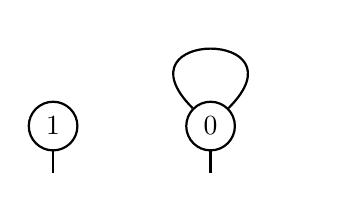
\begin{tikzpicture}[scale=1, transform shape, every loop/.style={}]
    \node[circle,draw=black,thick] (B) at (-1,0) {$1$};
    \draw[-,thick] (B) -- (-1,-0.6);
    \node[circle,draw=black,thick] (A) at (1,0) {$0$};
    \draw[-,thick] (A) -- (1,-0.6);
    \path[every node/.style={font=\sffamily\small},thick]
        (A)   edge[loop] (A);
    \end{tikzpicture}
    \end{center}
    \caption{Stable graphs for $g=1, n=1$}%
    \label{fig:03graphloop}
    \end{figure}
    The first graph $\Gamma_1$ gives us the contribution
    \begin{align*}
        \Cont_{\Gamma_1} &= T\omega_{1,1}^{\E}(R(z)^{-1}\1) \\
        &= \omega_{1,1}^{\E}(R(z)^{-1}\1) + p_* \omega_{1,1}^{\E}(R(z)^{-1}\1, T_R(z)).
    \end{align*}
    Using the formula $B_2 = \frac{1}{6}$ and the fact that $\dim \Mbar_{1,1} = 1$, this becomes
    \[ 1 - \frac{1}{12}\psi_1 + \frac{1}{12} \kappa_1. \]
    The second graph does not receive tail contributions because $\dim \Mbar_{0,3} = 0$. The constant term of the edge contribution is $\frac{1}{12}$, so considering the automorphism and pushing forward to $\Mbar_{1,1}$ gives us
    \[ \Cont_{\Gamma_2} = \frac{1}{12} \Delta, \]
    where $\Delta$ denotes the boundary divisor (with the correct stack structure). Because $\psi_1 = \kappa_1$ in this case, we obtain
    \[ 1+\lambda_1 = 1 + \frac{1}{12}(\kappa_1 - \psi_1 + \Delta) = 1 + \frac{1}{12} \Delta. \]
\end{exm}




\subsection{Operator formalism and geometric quantization}%
\label{sub:Operator formalism and geometric quantization}

We will return to the symplectic formalism of Givental. This is more convenient for certain computations, but it is in fact equal to what we have before, at least when we want to calculate generating functions. Recall that we had a Frobenius manifold structure on $V$ and we considered the vector space $\mc{V}\coloneqq V\ls{z^{-1}}$ with symplectic form
\[ (\mbf{f}(z), \mbf{g}(z)) \coloneqq \on{Res}_{z=0} \eta(\mbf{f}(-z), \mbf{g}(z)). \]
If we consider the polarization given by $\mc{V}_+ = V[z]$ and $\mc{V}_- = z^{-1}V\ps{z^{-1}}$, then letting $\bq$ be as before (with the dilaton shift), let $\bp$ be coordinates on $\mc{V}_-$ such that $(\bq, \bp)$ form a system of Darboux coordinates for $\mc{V}$.

\begin{defn}
    We will call any formal function of the form
    \[ \mc{D} = \exp\ab(\sum_{g=0}^{\infty} \hbar^{g-1} \mc{F}_g) \]
    an \textit{asymptotic element of the Fock space}.
\end{defn}

Then given such an asymptotic element of the Fock space, we will quantize (infinitesimal) symplectic transformations on $\mc{V}$ by the following formulae:
\[ \wh{p_a p_b} \coloneqq \hbar \partial_{q_a} \partial_{q_b}, \qquad \wh{p_a q_b} \coloneqq q_b \partial_{q_a}, \qquad \wh{q_a q_b} = \frac{q_a q_b}{\hbar}. \]
In particular, this will allow us to understand expressions like $\hat{R} \mc{D}$. However, we need to be careful because our formulae will involve both the fundamental solution $S_{\tau}$ and the $R$-matrix, and $S_{\tau}$ is a power series in $z^{-1}$.\footnote{This is because we expand $\frac{1}{z-\psi} = \sum_{n=0}^{\infty} \psi^n z^{-n-1}$.}

\begin{thm}[Givental {\cite{Givental2001quantization}}]
    An operator of the form $S(z^{-1}) = \mr{Id} + S_1 z^{-1} + \cdots$ acts on (asymptotic) elements of the Fock space by the formula
    \[ \hat{S}^{-1} \mc{D}(\bq) = e^{\frac{1}{2\hbar}W(\bq,\bq)} \mc{D}([S \bq]_+), \]
    where $W = \sum \eta(W_{mn}q_m, q_n)$ is defined by the formula
    \[ \frac{S(w^{-1})^* S(z^{-1}) - \mr{Id}}{w^{-1}+z^{-1}} = \sum \frac{W_{mn}}{w^m z^n}. \]
    Operators of the form $R(z) = \mr{Id} + R_1 z + \cdots$ act by the formula
    \[ \hat{R}\mc{D}(\bq) = e^{\frac{\hbar}{2} V(\partial_{\bq}, \partial_{\bq})} \mc{D}(R^{-1} \bq), \]
    where $V = \sum \eta(p_m, V_{mn} p_n)$ is defined by 
    \[ \frac{R(w)^* R(z) - \mr{Id}}{w+z} = \sum V_{mn} w^m z^n. \]
\end{thm}

For a semisimple CohFT, there is a system of \textit{canonical coordinates} $u_{\alpha}$ such that the $1$-form $\d{u}$ is a homomorphism of algebras $T_v V \to \C$. Then near a semisimple point, there is an asymptotic solution to the quantum connection of the form
\[ \Psi \cdot  R \cdot e^{\frac{U}{z}}, \]
where $\Psi$ switches from flat coordinates to canonical coordinates and $U = \on{diag}(u_{\alpha})$ is the matrix of canonical coordinates. Finally, define
\[ C = \frac{1}{2} \int^u \sum R_1^{\alpha\alpha} \d{u_{\alpha}}. \]
A corollary of Teleman's reconstruction theorem is the formula
\[ \mc{D}^X = e^{C(u)} \hat{S}^{-1}_{\tau} \hat{\Psi} \hat{R} \wh{e^{\frac{U}{z}}} \prod_{i=1}^{\dim V} \mc{D}^{\mr{pt}} \]
for the Gromov-Witten theory of any smooth projective variety with semisimple quantum cohomology.

\begin{exm}
    As a final example, we will apply Teleman's theorem to compute $F_1$ of any semisimple CohFT. Let $e_{\mu}$ denote an idempotent basis for the quantum product. We will compute
    \[ \int_{\Mbar_{1,1}} \Omega_{1,1}(e_{\beta}). \]
    Using the reconstruction theorem, we obtain
    \begin{align*}
        \int_{\Mbar_{1,1}}\Omega_{1,1}(e_{\beta}) ={}& \int_{\Mbar_{1,1}} T_R \omega_{1,1}(R(\bar{\psi})^{-1} e_{\beta}) + \frac{1}{2} T_R \omega_{0,3}(R(\bar{\psi})^{-1} e_{\beta}, V(\bar{\psi}_2, \bar{\psi}_3)) \\
        ={}& \int_{\Mbar_{1,1}}T_R\omega_{1,1}(e_{\beta}) - \int_{\Mbar_{1,1}} T_R \omega_{1,1}(R_1 e_{\beta})\bar{\psi} \\ 
        &+ \frac{1}{2}\sum_{\mu}  \omega_{0,3}(e_{\beta}, R_1 e^{\mu}, e_{\mu}) \\
        ={}& \int_{\Mbar_{1,1}} ( \omega_{1,1}(e_{\beta}) + p_* ( \omega_{1,2}(e_{\beta}, R_1 \1) \bar{\psi}_2^2 )) \\
        &- \int_{\Mbar_{1,1}} (\omega_{1,1}(R_1 e_{\beta})\bar{\psi}_1 + p_* ( \omega_{1,2}(R_1 e_{\beta}) \bar{\psi}_2^2 ) \bar{\psi}_1) \\
        &+ \frac{1}{2} \sum_{\mu} \eta(e_{\beta} \star e_{\mu}, R_1 e^{\mu}) \\
        ={}& \frac{1}{24} \sum_{\mu} ( \omega_{0,4}(e_{\mu}, e^{\mu}, e_{\beta}, R_1 \1) -\omega_{0,3}(e_{\mu}, e^{\mu}, R_1 e_{\beta}) )\\
        &+ \frac{1}{2} \eta(e_{\beta}, R_1 e^{\beta}) \\
        ={}& \frac{1}{24} \sum_{\mu}\sum_{\nu} \omega_{0,3}(e_{\mu}, e^{\mu}, e_{\nu})\omega_{0,3}(e^{\nu}, e_{\beta}, R_1 \1) \\
        &-\frac{1}{24} \sum_{\mu} \omega_{0,3}(e_{\mu}, e^{\mu}, R_1 e_{\beta}) + \frac{1}{2} (R_1)_{\beta\beta} \\
        ={}& \frac{1}{24} \ab(\eta(e^{\beta}, R_1 \1) - \sum_{\mu} \eta(e^{\mu}, R_1 e_{\beta})) + \frac{1}{2} (R_1)_{\beta\beta}.
    \end{align*}
    Using the identities
    \begin{align*}
        \eta(R_1 \1, e^{\beta}) - \sum_{\mu} \eta(R_1 e_{\beta}, e^{\mu}) &= \sum_{\mu} \Delta_{\mu} \int_{\Mbar_{0,4}} \Omega_{0,4}(e_{\mu}, e_{\mu}, e_{\mu}, e_{\beta}) \\
        &= -\frac{1}{2}\sum_{\mu} \Delta_{\mu} \partial_{u_{\beta}} \Delta_{\mu}^{-1} \\
        &= \frac{1}{2} \sum_{\mu} \partial_{u_{\beta}} \log \Delta_{\mu},
    \end{align*}
    where $\Delta_{\mu} \coloneqq \eta(e_{\mu}, e_{\mu})^{-1}$, we obtain the result
    \[ \int_{\Mbar_{1,1}} \Omega_{1,1}(e_{\beta}) = \frac{1}{48} \sum_{\mu} \partial_{u_{\beta}} \log \Delta_{\mu} + \frac{1}{2} (R_1)_{\beta\beta}, \]
    which can be placed in the suggestive form
    \[ \d{F_1^{\Omega}} = \sum_{\mu} \ab( \frac{\d{\log \Delta_{\mu}}}{48} + \frac{1}{2} (R_1)_{\mu\mu} \d{u_{\mu}} ). \]
    This recovers a result which was already known to Givental.
\end{exm}

\subsection{How to compute the R-matrix}%
\label{sub:How to compute the R-matrix}

We will conclude by explaining how to compute the R-matrix, starting in the setting where the Frobenius manifold is conformal (for example the Gromov-Witten theory of a smooth projective variety, \(r\)-spin curves, etc). In this example, we will consider the Frobenius manifold for 3-spin curves, following~\cite{PPZ2015}. Let \(V\) be 2-dimensional with coordinates \(x\) and \(y\), where \(x\) corresponds to the unit. The metric is given by
\[ \eta = \begin{pmatrix}
    0 & 1 \\
    1 & 0
\end{pmatrix} \]
and the primary genus zero potential is \(F(x,y) = \frac{1}{2} x^2 y + \frac{1}{72} y^4\). There is an \textit{Euler vector field}
\[ E = x \pdv{}{x} + \frac{2}{3} y \pdv{}{y}, \]
which acts with weights \(-1\) and \(-\frac{2}{3}\) on \(\partial_x\) and \(\partial_y\), respectively. The conformal dimension is \(\delta = \frac{1}{3}\), and we will define the degree operator
\[ \mu(v) = [E,v] + \ab(1 - \frac{\delta}{2})v. \]
Here, \(\partial_x\) has degree \(-\frac{1}{6}\) and \(\partial_y\) has degree \(\frac{1}{6}\).

To make our lives easier, we will set \(\phi = \frac{y}{3}\) and define
\[ \hat{\partial}_x = \phi^{1/4} \partial_x, \qquad \hat{\partial}_y = \phi^{-1/4} \partial_y, \]
and then compute in this frame. In this setting, quantum multiplication is given by
\[ \hat{\partial}_x \star \hat{\partial}_x = \phi^{1/4} \hat{\partial}_x, \qquad \hat{\partial}_x \star \hat{\partial}_y = \phi^{1/4} \hat{\partial}_y, \qquad \hat{\partial}_y \star \hat{\partial}_y = \phi^{1/4} \hat{\partial}_x. \]
The last thing we need is that quantum multiplication by \(E\) is given by
\[ E \star - = \begin{pmatrix}
    x & 2 \phi^{3/2} \\
    2 \phi^{3/2} & x 
\end{pmatrix}. \]
We will now compute the R-matrix \(R = 1 + R_1 z + \cdots\) by using the recursive equation
\[ [R_{k+1}, E \star -] = (k + \mu) R_k. \]
Setting \(R_k = \begin{psmallmatrix}
    a_k & b_k \\
    c_k & d_k
\end{psmallmatrix}\), we obtain the equation
\[ \ab[
    \begin{pmatrix}
        a_{k+1} & b_{k+1} \\
        c_{k+1} & d_{k+1}
    \end{pmatrix}, \begin{pmatrix}
        x & 2 \phi^{3/2} \\
        2 \phi^{3/2} & x 
    \end{pmatrix}
] = \frac{1}{6} \pdiagmat[empty={}]{6k-1, 6k+1} \begin{pmatrix}
    a_k & b_k \\
    c_k & d_k 
\end{pmatrix}. \]

The unique solution of this is in fact
\begin{align*}
    a_k &= \frac{1}{1728^k \phi^{3k/2}} \frac{1+6k}{1-6k} \frac{(6k)!}{(3k)!(2k)!} \delta_{k, \text{even}},  \\
    b_k &= \frac{1}{1728^k \phi^{3k/2}} \frac{1+6k}{1-6k}\frac{(6k)!}{(3k)!(2k)!} \delta_{k, \text{odd}},  \\
    c_k &= \frac{1}{1728^k \phi^{3k/2}}\frac{(6k)!}{(3k)!(2k)!} \delta_{k, \text{odd}}, \\
    d_k &= \frac{1}{1728^k \phi^{3k/2}} \frac{(6k)!}{(3k)!(2k)!} \delta_{k, \text{even}}. 
\end{align*}
If you are familiar with tautological relations on the moduli space of curves, you will see that the series \(a_k + b_k\) and \(c_k + d_k\) enter in the formulation of the Faber-Zagier relations and the formulation of Pixton's relations. 

In the case where the Frobenius manifold is not conformal (for example in equivariant Gromov-Witten theory), we will need to use an oscillating integral or some other technique to fix initial values in the R-matrix. We will give an example computation here, which is due to Givental~\cite{Givental2001semisimple}. In this setting, \(X = \P^n\), but the argument can be made to work for any Fano toric variety. Recall that the equivariant mirror of \(\P^n\) is the superpotential
\[ W = x_1 + \cdots + x_{n+1} + \sum_{i=1}^{n+1} \lambda_i \log x_i \]
(here, we change the sign of the equivariant parameters for convenience). Therefore, the oscillating integrals will look like
\[ I = \int_{\Gamma \subset E_q = (x_1 \cdots x_{n+1}=q)} e^{W/z} \prod_{i=1}^{n+1} \frac{\d{x_i}}{x_i}. \]
This is annihilated by the operator 
\[ \prod_{i=1}^{n+1}\ab(zq \odv{}{q} -\lambda_i) - q, \]
which is exactly the Picard-Fuchs equation satisfied by the I-function of projective space.

To expand this integral near the critical points, we first need to compute the critical points. Here, using coordinates \(t = \log q\) and \(T_i = \log x_i\), we obtain the equation
\[ x_i = L - \lambda_i, \]
where \(L\) is the Lagrange multiplier. These satisfy the equation
\[ \prod_{i=1}^{n+1} (L - \lambda_i) = q, \]
and therefore for generic values of \(\lambda\), near \(q = 0\), the possible values \(L_i\) of the Lagrange multiplier are distinguished by which of the \(\lambda_i\) they begin with. Note that the function \(W\), the values of the Lagrange multipliers, and therefore the critical points, all depend continuously on \(\lambda\), so they admit non-equivariant limits at \(\lambda = 0\) when \(q \neq 0\).

When \(q = 0\), the matrix \(\Psi\) transitions from the flat basis \(\ab{H^i}\) to the basis
\[ L_i(H) = \prod_{j \neq i} \frac{H - \lambda_j}{(\lambda_i - \lambda_j)^{1/2}}, \]
which are the leading terms of the canonical coordinates (simply compute the fixed points of the torus action via equivariant localization, and we will obtain this Lagrange interpolation). Therefore, we need to compute \(L_j \ab(z q \odv{}{q}) I\) in the \(q = 0\) limit. A direct computation shows that applying \(L_i \ab(z q \odv{}{q})\) to the integral introduces an additional factor proportional to \(\frac{q}{x_i}\) to the integrand of the oscillating integral. Because we can permute the indices, we will compute only the case where \(i = n+1\). Another direct computation shows that the integral vanishes at \(q = 0\) unless \( j = n+1\), so in fact we see that \(R\) is diagonal in the classical limit. When \(j = n+1\), we have
\[ \frac{q}{x_{n+1}} = x_1 \cdots x_n, \]
and the integral becomes
\[ \int_{\Gamma} e^{\ab( \sum_{i=1}^n x_i + (\lambda_i - \lambda_{n+1})\log x_i ) / z} \d{x_1} \cdots \d{x_n} = \prod_{i=1}^n \int_{\R} e^{x_i/z} x_i^{(\lambda_i - \lambda_{n+1})/z} \d{x_i}, \]
which is simply a product of gamma functions.

\begin{lem}
    We have the asymptotics
    \[ \log \Gamma(1+s) \sim s \log \ab(\frac{s}{e}) + \frac{1}{2} \log(2\pi s) + \sum_{k=1}^{\infty} \frac{B_{2k}}{2k} \frac{s^{1-2k}}{2k-1}. \]
\end{lem}
Using this, we see that at \(q = 0\), the diagonal matrix element of the R-matrix is given by
\[ \log R = \sum_{k=1}^{\infty} \frac{B_{2k}}{2k} \frac{z^{2k-1}}{2k-1} \sum_{i =1}^n (\lambda_i - \lambda_{n+1})^{1-2k}. \]
By a result of Givental, this implies that this R-matrix recovers the equivariant GW theory of \(\P^n\), and as a corollary, because the non-equivariant limit exists, we obtain Virasoro constraints for \(\P^n\). 

